\input preamble.tex
\begin{centering}
\Huge{\textbf{Høstprøve 01}}\\
\end{centering}
\vskip 2cm 
\begin{itemize}
	%\item utføre arbeid på automatiserte anlegg fagmessig, nøyaktig og i overensstemmelse med krav til helse, miljø og sikkerhet og rutiner for kvalitetssikring og internkontroll
	%\item utføre risikovurdering og vurdere tiltak for ivaretakelse av person– og maskinsikkerhet
	%\item vurdere hvilke regelverk og normer som gjelder for arbeidet som skal utføres og anvende dette
	\item planlegge, utføre, vurdere kvalitet, sluttkontrollere og dokumentere arbeidet
	\item planlegge, programmere, montere og idriftsette programmerbare styresystemer
	\item endre og tilpasse skjermbilder for grensesnitt mellom menneske og maskin
	\item anvende ulike elektroniske kommunikasjonssystemer i automatiserte anlegg
	%\item vurdere datasikkerhet i automatiserte anlegg
	\item tegne, lese og forklare instrumenterte prosessflytskjemaer og bruke annen relevant dokumentasjon for automatiserte anlegg
	\item montere, konfigurere, kalibrere og idriftsettelse digitale og analoge målesystemer
	%\item idriftsette og optimalisere regulatorer basert på prosessbehov
	%\item montere og idriftsette ulike typer pådragsorganer med tilhørende forstillingselementer og hjelpeutstyr
	%\item programmere, idriftsette samt gjøre rede for roboters funksjon og anvendelse i produksjonsanlegg
	%\item måle fysiske størrelser i automatiserte anlegg
	%\item feilsøke og rette feil i automatiserte anlegg
	%\item bruke gjeldende regelverk og normer for elektriske installasjoner på maskiner
	%\item bruke gjeldende regelverk og normer for installasjon av elektroniske kommunikasjonssystemer
	%\item beskrive ulike vedlikeholdssystemer og -rutiner knyttet til automatiserte anlegg, og anvende et av disse
	%\item redegjøre for bedriftens organisasjonsoppbygging og bedriftens verdiskapning i et samfunnsperspektiv
	%\item dokumentere egen opplæring i automatiseringssystemer
\end{itemize}
\vskip 2.5pt 
Hjelpemidler:\begin{itemize}[noitemsep]
	\item Oppgave 1-4: Kalkulator og formelark
	\item Oppgave 5-9 Alle ikke kommuniserende
\end{itemize}

\vskip 5pt 
\vskip 10pt 
Alle ark som leveres inn skal ha elevens navn.
\vskip 2.5pt 
Oppgave 1-4 skal leveres på papir, etter levering kan eleven ta frem PC og svare på oppgave 9. 
\vskip 2.5pt 
Oppgave 5-9 skal utføres i samme codesys project. (slik at det bare leveres inn en fil.)
Når oppgave 5-9 skal leveres kan elevene slå på trådløst nettverkt og sende oppgaven på mail til:
\vskip 2.5pt 
fred-olav.mosdal@skole.rogfk.no
\vskip 2.5pt 
I emnefeltet skal det stå: PLS Prøve
\vskip 2.5pt
Oppgaven SKAL sendes fra skolemailen. 
\vskip 2cm   
Konaktinformasjon:
\begin{itemize}[noitemsep]
	\item Kontaktlærer: Fred-Olav Mosdal
	\item TLF: 90507684
\end{itemize}


\vfil \eject
%Slutt forside
Oppgave 1 (6p)%Navngi
\vskip 2.5pt 
En forbedring i forhold til endebrytere med fysisk kontakt kan i mange tilfeller være induktive nærhetssensorer. Denne type bryter aktiveres ved at et objekt kommer nærme den. Det er ikke nødvendig med fysisk kontakt. Forklar hvordan denne type bryter virker, og hvilke materialer den kan detektere. 

Induktive nærhetssensorer trenger driftsspenning. Det er vanlig med +24V DC. Utgangen er normalt ikke en potensialfri kontakt, men en transistor. 

$$\includegraphics[width=15.5cm]{i02243x01.eps}$$

\vskip 30pt

Vis hvordan du ville koblet kretsen nedenfor slik at LED-en lyser når sensoren aktiveres. Anta at utgangen er sourcing (PNP).
Oppgave 2 (6p) %Definisjoner
\vskip 2.5pt 
a) Hva en en transission i sekvensielle funknsjonskart?\\
\vskip 2.5pt 

\begin{tikzpicture}
	\draw[step=0.5cm,gray!20,thin]  grid (17,11) ;
\end{tikzpicture}
\vskip 10pt 
b) Hva er en action i sekvensielle funksjonskart?\\
\vskip 2.5pt 

\begin{tikzpicture}
	\draw[step=0.5cm,gray!20,thin]  grid (17,11) ;
\end{tikzpicture}
\vskip 2.5pt 
\vskip 2.5pt 
\vfil\eject

Oppgave 3 (6p)%Enkel utregninger.
\vskip 2.5pt 
En Allen-Bradley SLC500 PLS blir bukt som regulator for en ovn. Prosessvariabelen TT01 er tilkoblet channel 0 på en firekanals inngangmodul. Transmitteren har et måleområde på 100-600°C. Vi må skallere denne verdien slik at den kan brukes til å gengi temperaturen på på HMI. HMI symbolet som skal brukes skal tilføres en verdi på 1000-6000. Komma tilføres automatisk av symbolet.  


$$\includegraphics[width=15.5cm]{i03648x01.eps}$$

Prosessbildet forteller at inngangmodulen gir en int verdi på 4000 ved 4mA og 20000 ved 20mA. 

\vskip 10pt
\vfil\eject
a) Lag en matematisk formel for konverteringen av temperaturen. 
\vskip 10pt

\begin{tikzpicture}
	\draw[step=0.5cm,gray!20,thin]  grid (17,11) ;
\end{tikzpicture}
\vskip 10pt 
b) tegn et ladder program som viser hvordan denne formelen kan implementeres. 

\vskip 10pt 

\begin{tikzpicture}
	\draw[step=0.5cm,gray!20,thin]  grid (17,11) ;
\end{tikzpicture}
\vfil\eject
Oppgave 4 (6p) %Tegneoppgaver(blokkskjema skisse osv. 
Suppose we have a Koyo ``CLICK'' PLC connected to three pushbutton switches as shown in this illustration:

$$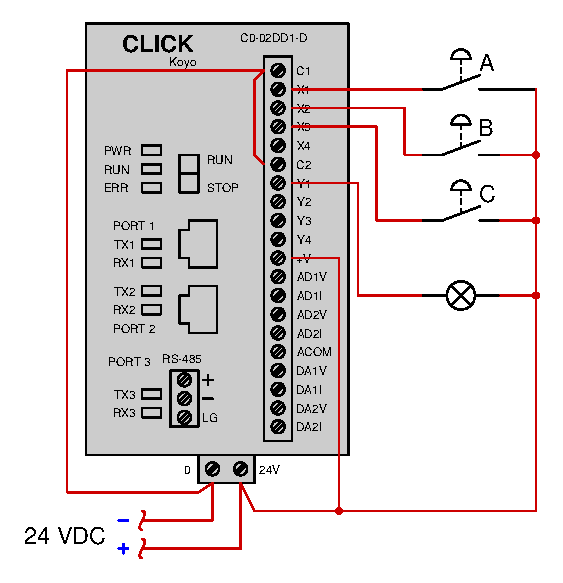
\includegraphics[width=15.5cm]{i04666x01.eps}$$

Determine the switch actuation statuses (i.e. pressed versus released) given the ``live'' display of the ladder logic program shown here:

$$\includegraphics[width=15.5cm]{i04666x02.eps}$$

Also, determine the status of the lamp connected to the PLC's {\tt Y1} output.
% Her kommer oppgaver som skal kreve forklaringer eller forståelse
\vfil\eject
Oppgave 5 (6p) %Kombinatorisk programmering

\vskip 2.5pt 
Oppgave 5 til 8 bygger på hverandre.
\vskip 2.5pt
 Tegningen nedenfor viser anlegget det er snakk om. Det skal lages en HMI som gjør det mulig å teste programmet. Det vil si at alle brytere, lamper og informasjon må vises på HMI. 
 \vskip 10pt 
$$\includegraphics[width=16cm]{aStyring01x01.eps}$$
\vskip 10pt 
Lag et program for Start og Stopp av transportbåndet. Transport båndet skal også stopppe ved manglende klar signal fra sikkerhetsrelaterte deler av styresystemet. 

\vskip 10pt 
Oppgave 6 (6p) % Tegn og forklar virkemåte
\vskip 2.5pt 
Legg til forsinket start på 3s av transportbåndet 

\vskip 10pt 
Oppgave 7 (6p) % Tegn og forkalr virkemåte. 
\vskip 2.5pt 
Når esken er full (10 deler), skal transportbåndet stoppe og det skal gis signal om at eske er full

\vskip 10pt 
Oppgave 8 (6p) % Regneoppgave
\vskip 2.5pt 
Om det ikke er registrert ny del på 15s skal transportbåndet stoppe og et varsellys aktiveres. 
\vskip 1cm

\vskip 5pt 
\vskip 0.5cm


\vfil\eject
Oppgave 9 (12p) \\ %skal beskrive hvordan en jobb skal utføres. (Planlegg, besriv hvordan du ville gjenomført og dokumenter jobben)
Oppgave med montering av transmitter og presentasjon av data på HMI

\vskip 5pt 
\includepdf[pages=-,angle=90]{../eq/afgvformler.pdf}
\end {document}
